\par Le membre du groupe responsable de cette partie était Antoine Vallée.

\subsubsection{Menu}
\par Le menu est une étape indispensable dans la création d'un jeu vidéo. Nous avons décidé de baser le notre sur un système de pile: Chaque scène s'empile les unes par dessus les autres, ainsi au plus bas de la pile vous aurez toujours le menu du départ, puis s'empile par dessus le choix du mode de jeu, le choix du niveau, pour finir sur la scène de jeu.
\par La pause s'empile encore par dessus la scène de jeu, puis tout est dépilé quand besoin pour revenir au menu principal. Le menu était présent très rapidement dans le jeu, car nous souhaitions le terminer avant de trop avancer dans le développement du jeu en lui même, c'est pourquoi ce dernier n'a pas changé d'aspect graphique depuis la soutenance 2.
\par Une capture d'écran du menu:

\begin{center}
	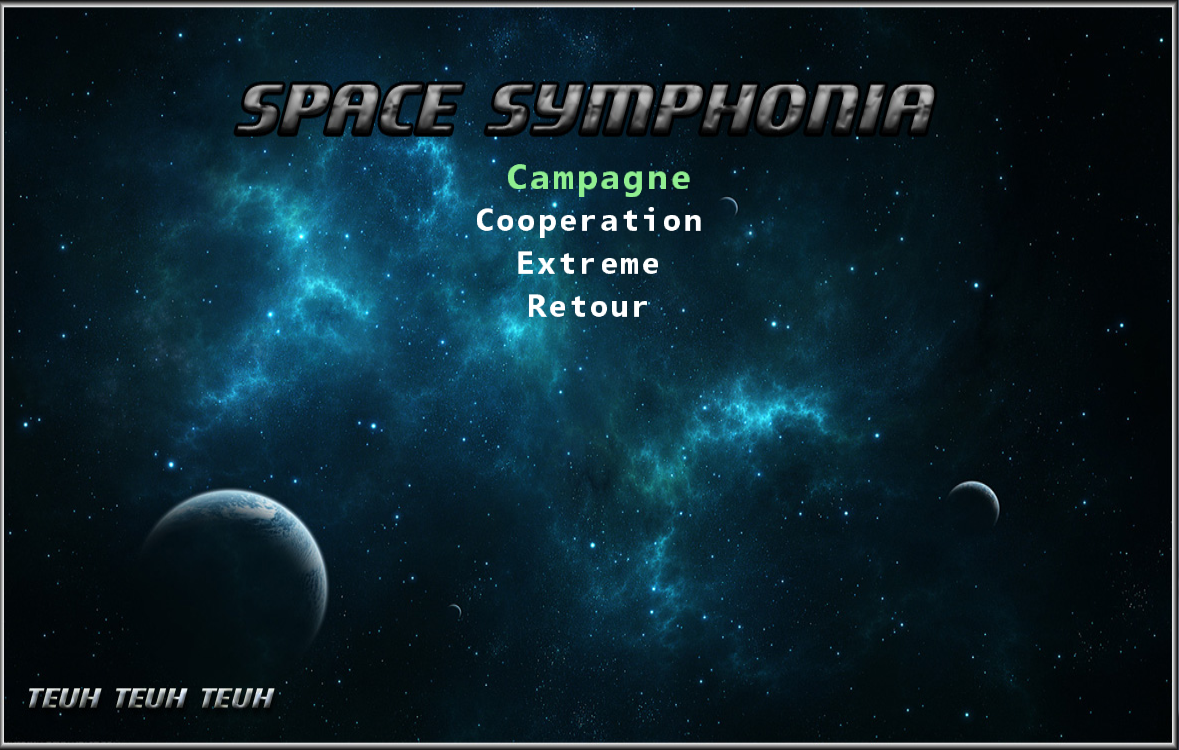
\includegraphics[width=13cm]{images/menu1.png}
\end{center}

\par Le menu permet donc au joueur d'accéder directement au jeu, mais aussi d'ouvrir l'éditeur de niveau afin de créer ses propres niveaux, de changer la difficulté du jeu, de voir ses scores.

\subsubsection{Scores}
\par Dans un Shoot Them All, le score est surement ce qu'il y a de plus important. Nous devions développer un système infaillible et performant, dans lequel le joueur pourrait se comparer à ses amis.
\par Ainsi, à chaque fin de niveaux, en mode campagne ou extrême, le joueur est invité à rentrer son nom. Son score est enregistré, et est visible dans le menu partie "Scores". 
\par Dans ce menu, tous les meilleures scores par niveaux sont d'abord affichés. Le joueur peut ensuite se déplacer sur le niveau dont il souhaite obtenir plus de détails concernant les scores, pour voir l'ensemble des scores effectués sur ce niveau.

\begin{center}
	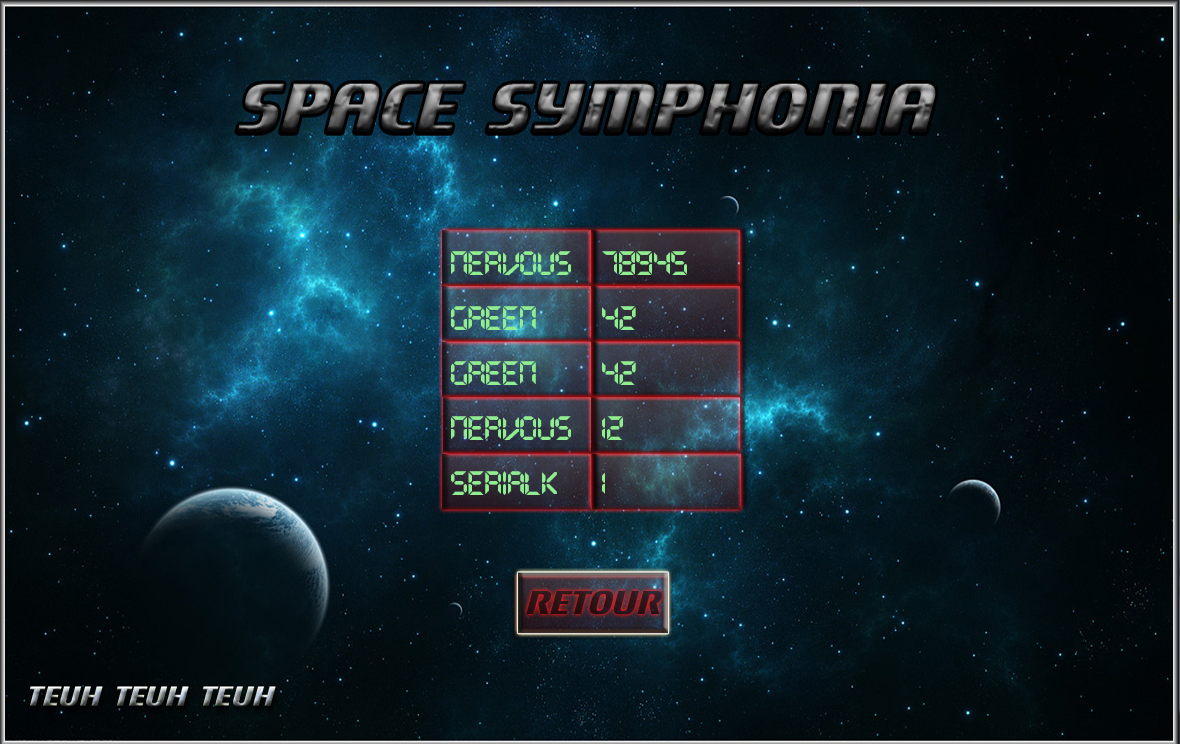
\includegraphics[width=13cm]{images/score1.png}
\end{center}